\documentclass[letter,twoside,10pt]{article}
\usepackage{tutorial}
\graphicspath{{figs/}}
\def\figurename{Figure}
\def\tablename{Tableau}
\newcommand{\italic}[1]{\emph{#1}} 

% ------------------------------------------------------------------------
\newcommand\IL{{\itshape left}}
\newcommand\IR{{\itshape right}}
\newcommand\IM{{\itshape middle}}
\newcommand\IT{{\itshape top}}
\newcommand\IB{{\itshape bottom}}

% ------------------------------------------------------------------------
\newcommand{\CodeFmt}[1]{{\small\texttt{#1}}}

\def\kernel{\CodeFmt{Kernel}}

\def\cgalpoly{\CodeFmt{CGAL::Polyhedron\_3}}
\def\poly{\CodeFmt{Polyhedron\_3}}
\def\polytrait{\CodeFmt{PolyhedronTraits\_3}}
\def\polyitem{\CodeFmt{PolyhedronItems\_3}}
\def\polybuilder{\CodeFmt{Polyhedron\_incremental\_builder\_3}}

\def\cgalhds{\CodeFmt{CGAL::HalfedgeDS}}
\def\hds{\CodeFmt{HalfedgeDS}}
\def\hdsitem{\CodeFmt{PolyhedronItems}}

% L.K. -------------------------------------------------------------------
\newcommand{\CC}{C\raise.08ex\hbox{\texttt{++}}}
\newcommand{\openmesh}{\textsc{OpenMesh}}
\newcommand{\opensg}{\textsc{OpenSG}}
\newcommand{\cgal}{\textsc{Cgal}}
\newcommand{\stl}{\textsc{Stl}}


% hyperref stuff
\usepackage{hyperref}
\hypersetup{
  pdftitle={Getting started with CGAL Polyhedron},
  pdfauthor={INRIA Geometrica},
  pdfsubject={A tutorial for CGAL},
  pdfkeywords={},
  pdfpagemode=UseThumbs,
  baseurl={http://www.cgal.org},
  colorlinks=true,
  linkcolor=black,
  anchorcolor=black,
  citecolor=black,
  filecolor=black,
  menucolor=black,
  pagecolor=black,
  urlcolor=blue,
  bookmarksopen=false,}
% end hyperref stuff


\begin{document}

% TITLE
\date{}
\title{{\LARGE {\sffamily\bfseries Getting started with CGAL
Polyhedron}}\\ the example of subdivision surfaces}
\author{
\sffamily Pierre Alliez\footnote{GEOMETRICA, INRIA Sophia-Antipolis}
\and 
\sffamily Andreas Fabri\footnote{GeometryFactory, Sophia-Antipolis}
\and 
\sffamily Lutz Kettner\footnote{Max-Planck Institut f�r Informatik, 
                                Saarbr�cken}
\and
\sffamily Le-Jeng Shiue\footnote{SurfLab, University of Florida}
\and
\sffamily Radu Ursu\footnote{GEOMETRICA, INRIA Sophia-Antipolis}}
\maketitle

\thispagestyle{empty}

% ABSTRACT

\abstract{This document gives a description for a user to get
started with the halfedge data structure provided by the Computational
Geometry Algorithm Library (CGAL). Assuming the reader to be familiar
with the C++ template mechanisms and the key concepts of the Standard
Template Library (STL), we describe three different approaches with
increasing level of sophistication for implementing mesh subdivision
schemes. The simplest approach uses simple Euler operators to
implement the $\sqrt{3}$ subdivision scheme applicable to triangle
meshes. A second approach overloads the incremental builder already
provided by CGAL to implement the quad-triangle subdivision scheme
applicable to polygon meshes. The third approach is more generic and
offers an efficient way to design its own subdivision scheme through
the definition of rule templates. Catmull-Clark, Loop and Doo-Sabin
schemes are illustrated using the latter approach. Two companion
applications, one developed on Windows with MS .NET, MFC and OpenGL,
and the other developed for both Linux and Windows with Qt and OpenGL,
implement the subdivision schemes listed above, as well as several
functionalities for interaction, visualization and raster/vectorial
output.}

\vskip 3mm

\noindent {\bf Keywords:}
                 CGAL library,
                 tutorial,
                 halfedge data structure, 
                 polygon surface mesh,
                 subdivision surfaces,
                 quad-triangle,
                 $\sqrt{3}$,
                 Loop,
                 Doo-Sabin,
                 Catmull-Clark,
                 OpenGL.

% INTRODUCTION                 
\section{Introduction}

% introduction to cgal

The CGAL library is a joint effort between nine European
institutes~\cite{fgkss-dccga-00}. The goal of CGAL is to make
available to users in industry and academia some efficient solutions
to basic geometric problems developed in the area of computational
geometry in a C++ software library.\\

% motivations

CGAL features a 3D polygon surface mesh data structure based on the
concept of halfedge data structure~\cite{k-ugpdd-99}, which has been
very successful for the design of general algorithms on meshes. In
this document we provide a tutorial to get started with CGAL
Polyhedron data structure through the example of subdivision
surfaces. We also offer an application both under windows and linux,
featuring an OpenGL-based viewer, an arcball for interaction and two
ways (raster and vectorial) to produce pictures and illustrations.\\

% teaser

\begin{figure}[htb]
    \centering{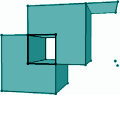
\includegraphics[width=\linewidth]{figs/teaser}}
    \caption{Snapshot taken from the tutorial application running
             on Windows. A polygon mesh is subdivided using the
             quad-triangle subdivision scheme~\cite{sl-qts-02}.}
    \label{fig:teaser}
\end{figure}
        

% targeted audience ?

The main targeted audience is a master or a Ph.D. student in computer
graphics or computational geometry, aiming at doing some research on
mesh processing algorithms. We hope this tutorial will convince the
reader~:

\begin{itemize}

\item 
not reinventing the wheel. Taking some time choosing the ``right
tool'' is often worth it. This may true, even for a short project;

\item 
using an optimized and robust library to ease the implementation and
obtain fast and robust results. This allows focusing on the elaborated
algorithm, not on the underlying data structure;

\item 
using generic programming to reuse existing data structures
and algorithms;

\item 
using a standard library in order to benefit from existing support and
discussion groups\footnote{see the cgal discuss list:
\href{http://www.cgal.org/user_support.html}
{http://www.cgal.org/user\_support.html.}}.

\end{itemize}               

% PREREQUISITES
\section{Prerequisites}

% C++ and generic programming

Before using CGAL, it is mandatory to be familiar with C++ and the
\italic{generic programming paradigm}. The latter features the notion
of C++ class templates and function templates, which is at the corner
stone of all features provided by CGAL.\\

% STL

An excellent example illustrating generic programming is the Standard
Template Library (STL)~\cite{ms-stl-96}. Generality and flexibility is
achieved with a set of \italic{concepts}, where a concept is a well
defined set of requirements. One of them is the \italic{iterator}
concept, which allows both referring to an item and traversing a
sequence of items. Those items are stored in a data structure called
\italic{container} in STL. Another concept, so-called
\italic{circulator}, allows traversing some circular sequences. They
share most of the requirements with iterators, except the lack of
past-the-end position in the sequence. Since CGAL is strongly inspired
from the genericity of STL, it is important to become familiar with
its concepts before starting using it.

% HALFEDGE DATA STRUCTURE
\section{Halfedge data structure}

The specification of a polygon surface mesh consists of combinatorial
entities: vertices, edges, and faces, and numerical quantities:
attributes such as vertex positions, vertex normals, texture
coordinates, face colors, etc. The \italic{connectivity} describes the
incidences between elements and is implied by the topology of the
mesh. For example, two vertices or two faces are adjacent if there
exists an edge incident to both.\\

% definition

A \italic{halfedge data structure} is an edge-centered data structure
capable of maintaining incidence informations of vertices, edges and
faces, for example for planar maps, polyhedra, or other orientable,
two-dimensional surfaces embedded in arbitrary dimension. Each edge is
decomposed into two halfedges with opposite orientations. One incident
face and one incident vertex are stored in each halfedge. For each
face and each vertex, one incident halfedge is stored (see
Fig.\ref{fig:halfedge}).

% halfedge

\begin{figure}[htb]
    \centering{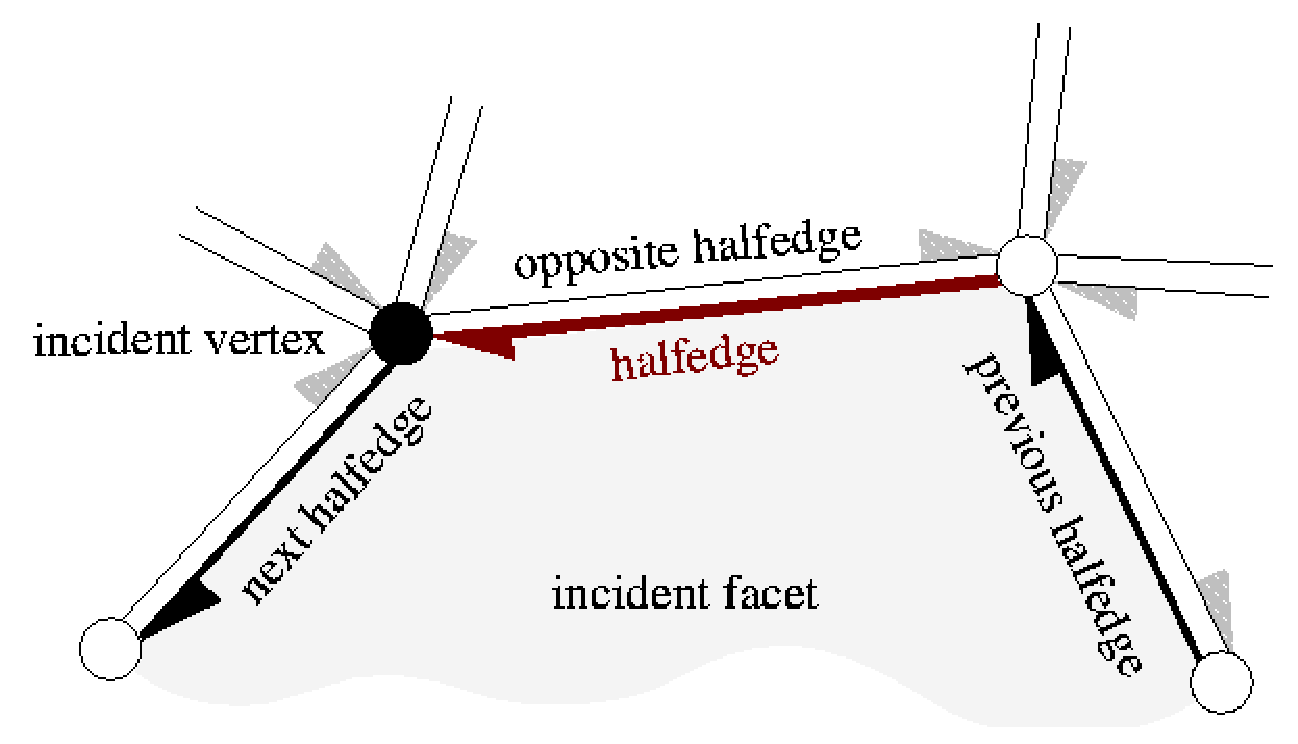
\includegraphics[width=\linewidth]{figs/halfedge}}
    \caption{One halfedge and its incident primitives.}
    \label{fig:halfedge}
\end{figure}
        
Notice that the halfedge data structure is only a combinatorial data
structure, geometric interpretation being added by classes built on
top of the halfedge data structure. On example is the class
\italic{CGAL::Polyhedron\_3} used in this tutorial. The 
halfedge data structure has been very successful for the design of
algorithms on meshes for several reasons:

\begin{itemize}

\item 
an edge-based data structure leads to a constant size structure,
contrary to face-based data structures with inevitable variable
topological structure when dealing with arbitrary vertex valence and
face degrees.

\item 
a halfedge encodes the orientation of an edge, facilitating the mesh
traversal.

\item 
navigation around each vertex by visiting all surrounding edges or
faces is made easy.

\item
each halfedge can be associated with a unique corner, that is a couple
$\{$face,vertex$\}$. The storage of attributes such as normals or
texture coordinates per corner (instead of per vertex) is thus
allowed.

\end{itemize}

% POLYHEDRON DATA STRUCTURE
\section{Polyhedron Data Structure}
\label{sec:polyhedron}

The class \verb+Polyhedron_3+ can represent polygon
meshes\footnote{\href{http://www.cgal.org/Manual/doc_html/basic_lib/Polyhedron_ref/Class_Polyhedron_3.html}{http://www.cgal.org}}.
Its underlying combinatorial component is based on the halfedge data
structure. As all CGAL geometric entities, its geometric component is
templated by the
\italic{kernel}\footnote{\href{http://www.CGAL.org/Manual/doc_html/frameset/fsKernel.html}{CGAL kernel}}.


\subsection{Declaration}

The simplest declaration of the polyhedron (without extended
primitives) consists of templating with a cartesian kernel and double
number precision:

{ \scriptsize
\begin{verbatim}
// instanciation of a polyhedron

#include <CGAL/Cartesian.h>
#include <CGAL/Polyhedron_3.h>

typedef CGAL::Cartesian<double>     kernel;
typedef CGAL::Polyhedron_3<kernel>  Polyhedron;

Polyhedron p;
\end{verbatim}}

\subsection{Extending primitives}

The polyhedron can be parameterized by a \italic{traits} class in
order to extend the vertex, halfedge and facet primitives. In this
tutorial all primitives (facets, halfedges and vertices) are
extended. The facet is extended with a normal and with a
general-purpose integer tag:

{ \scriptsize
\begin{verbatim}

template <class	Refs, class T, class P, class Norm>
class Enriched_facet : 
  public CGAL::HalfedgeDS_face_base<Refs, T>
{
  // tag
  int m_tag;

  // normal
  Norm m_normal;

public:

  // no  constructors to  repeat,  since  only
  // default constructor mandatory
  Enriched_facet()
  {
  }

  // tag
  const int&  tag()  {  return m_tag;  }
  void tag(const int& t)  {  m_tag  =  t; }

  // normal
  typedef  Norm Normal_3;
  Normal_3&  normal() { return  m_normal;  }
  const  Normal_3&  normal() const { return  m_normal;  }
};
\end{verbatim}}

The halfedge is extended with a general-purpose tag and a binary tag
to indicate wether it belongs to the control mesh or not. The latter
tag is used to superimpose the control mesh as shown in
Fig.\ref{fig:teaser}.

{ \scriptsize
\begin{verbatim}

template <class  Refs, class Tprev, class Tvertex, 
          class Tface, class Norm>
class Enriched_halfedge : public 
  CGAL::HalfedgeDS_halfedge_base<Refs,Tprev,Tvertex,Tface>
{
private:

  // tag
  int  m_tag; 

  // option  for control edge superimposing
  bool m_control_edge; 

public:

  // life  cycle
  Enriched_halfedge()
  {
    m_control_edge = true;
  }

  // tag
  const int& tag() const { return m_tag;  }
  int& tag() { return m_tag;  }
  void tag(const int& t)  {  m_tag  =  t; }

  // control edge  
  bool& control_edge()  { return m_control_edge; }
  const bool& control_edge()  const { return m_control_edge; }
  void control_edge(const bool& flag) { m_control_edge  =  flag;  }
};

\end{verbatim}}

The vertex is extended with a normal and a general-purpose integer
tag:

{ \scriptsize
\begin{verbatim}


template <class  Refs, class T, class P, class Norm>
class Enriched_vertex :  
  public CGAL::HalfedgeDS_vertex_base<Refs, T, P>
{
  // tag
  int  m_tag; 

  // normal
  Norm m_normal;

public:
  // life  cycle
  Enriched_vertex() {}
  // repeat  mandatory  constructors
  Enriched_vertex(const  P& pt)
    :  CGAL::HalfedgeDS_vertex_base<Refs, T,  P>(pt)
  {
  }

  // normal
  typedef  Norm Normal_3;
  Normal_3&  normal() { return  m_normal;  }
  const  Normal_3&  normal() const { return  m_normal;  }

  // tag
  int& tag() {  return m_tag;  }
  const int& tag() const {  return m_tag;  }
  void tag(const int& t)  {  m_tag  =  t; }
};

\end{verbatim}}



A redefined items class for the polyhedron uses the class wrapper
mechanism to embedd all three extended primitives within one unique
class.

{ \scriptsize
\begin{verbatim}

struct Enriched_items : public CGAL::Polyhedron_items_3
{
    // wrap  vertex
    template <class  Refs,  class  Traits>
    struct Vertex_wrapper
    {
        typedef  typename Traits::Point_3  Point;
        typedef  typename Traits::Vector_3  Normal;
        typedef  Enriched_vertex<Refs,
                          CGAL::Tag_true,
                          Point,
                          Normal>  Vertex;
    };

    // wrap  face
    template <class  Refs,  class  Traits>
    struct Face_wrapper
    {
        typedef  typename Traits::Point_3  Point;
        typedef  typename Traits::Vector_3  Normal;
        typedef  Enriched_facet<Refs,
                         CGAL::Tag_true,
                         Point,
                         Normal> Face;
    };

    // wrap  halfedge
    template <class  Refs,  class  Traits>
    struct Halfedge_wrapper
    {
        typedef  typename Traits::Vector_3  Normal;
        typedef  Enriched_halfedge<Refs,
                            CGAL::Tag_true,
                            CGAL::Tag_true,
                            CGAL::Tag_true,
                            Normal>  Halfedge;
    };
};
\end{verbatim}}

The trait class is then used for templating a polyhedron
\italic{Enriched\_polyhedron}:

{ \scriptsize
\begin{verbatim}

template <class  kernel,  class  items>
class  Enriched_polyhedron :
  public CGAL::Polyhedron_3<kernel,items>
{
  //...
};
\end{verbatim}}

The corresponding instanciation of an enriched polyhedron follows:

{ \scriptsize
\begin{verbatim}

#include <CGAL/Simple_cartesian.h>
#include "enriched_polyhedron.h"

typedef double number_type;
typedef CGAL::Simple_cartesian<number_type> kernel;

Enriched_polyhedron<kernel,Enriched_items> polyhedron;

\end{verbatim}}



\subsection{Iteration and Circulation}

The \italic{iterator} STL concept allows traversing a sequence of
items. This concept is applied to the primitives of a mesh, be they
halfedges, edges, vertices, facets or points. Notice that the order of
iteration is not dictated by any incidence relationship, contrary to
the circulator. The following example shows how to iterate on the mesh
vertices.

{ \scriptsize
\begin{verbatim}
Vertex_iterator iter;
for(iter = polyhedron.vertices_begin();
    iter != polyhedron.vertices_end();
    iter++)
{
  Vertex_handle hVertex = iter;
  // do something with hVertex
}
\end{verbatim}}

The \italic{circulator} STL concept allows traversing a circular
sequence of items. This concept is applied both inside facets and
around vertices. 

\paragraph{Circulating around a facet}
The facets being defined by the circular sequence of halfedges along
their boundary, this calls for a circulator around a facet. The
convention is that the halfedges are oriented counterclockwise around
facets as seen from the outside of the polyhedron (see
Fig.\ref{fig:stl_concept}, left).

{ \scriptsize
\begin{verbatim}
// circulate around hFacet
Halfedge_around_facet_circulator circ = hFacet->facet_begin();
Halfedge_around_facet_circulator end = circ;
CGAL_For_all(circ,end)
{
  Halfedge_handle hHalfedge = circ;
  // do something with hHalfedge
}
\end{verbatim}}

\paragraph{Circulating around a vertex}
The convention being that the halfedges are oriented counterclockwise
around facets as seen from the outside of the polyhedron, this implies
that the halfedges are oriented clockwise around the vertices (see
Fig.\ref{fig:stl_concept}, right).

{ \scriptsize
\begin{verbatim}
// circulate around hVertex
Halfedge_around_vertex_circulator circ = hVertex->vertex_begin();
Halfedge_around_vertex_circulator end = circ;
CGAL_For_all(circ,end)
{
  Halfedge_handle hHalfedge = circ;
  // do something with hHalfedge
}
\end{verbatim}}

% circulation inside a facet and around a vertex
\begin{figure}[htb]
    \centering{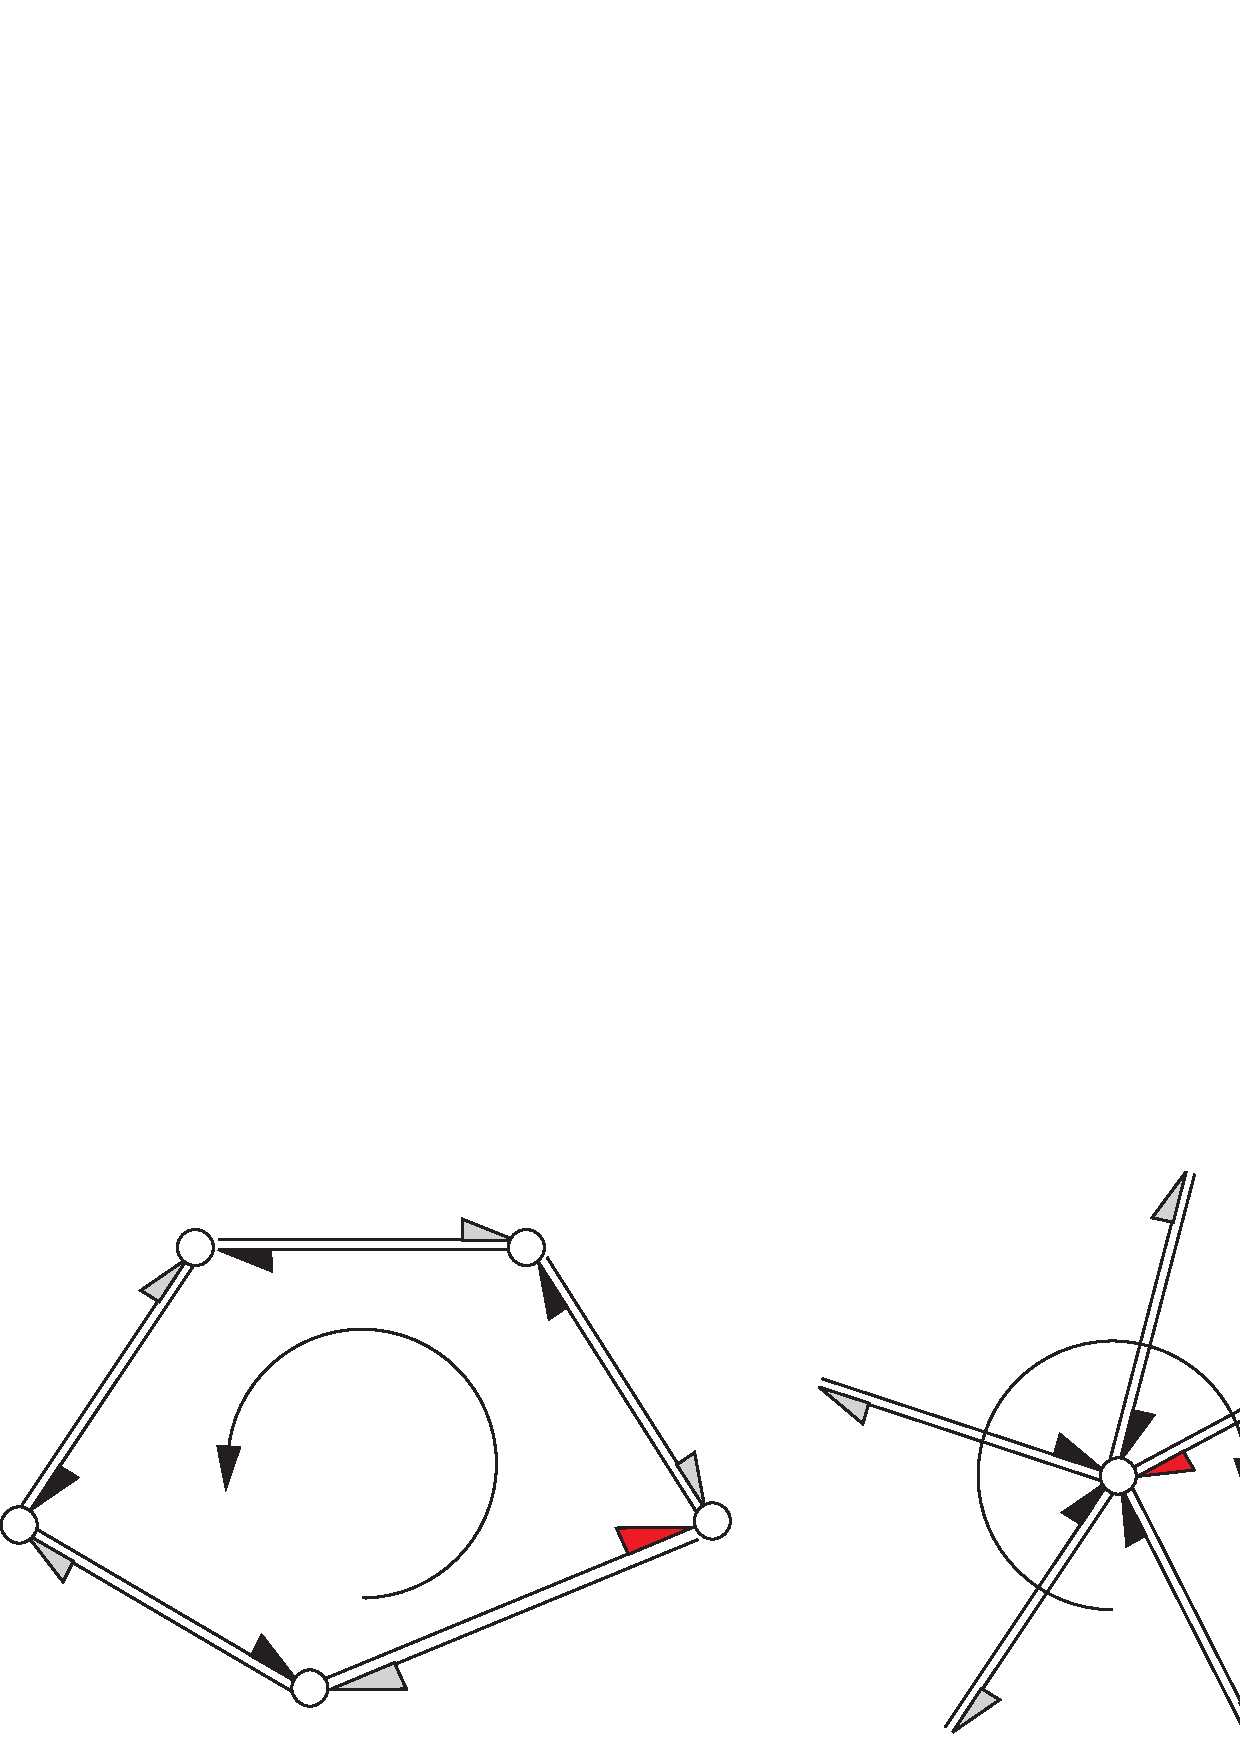
\includegraphics[width=\linewidth]{figs/stl_concepts}}
    \caption{Left: circulation around a facet (ccw).
             Right: circulation around a vertex (cw).}  
    \label{fig:stl_concept}
\end{figure}

\subsection{Mesh Editing}

The polyhedron provides a series of atomic operators to modify the
connectivity of the polyhedral surface:
\begin{itemize}
\item split or join of two facets,
\item split or join of two vertices,
\item split or join of two loops,
\item split of an edge.
\end{itemize}

Furthermore, more operators are provided to work with surfaces with
boundaries, to create or delete holes, add a facet to the border,
etc. We refere to the references manual for precise definitions and
illustratives figures\footnote{See
\href{http://www.cgal.org/Manual/doc_html/basic_lib/Polyhedron/Chapter_main.html}{Euler 
operators}}.

\subsection{Incremental Builder}
\label{sec:builder}


A utility class \verb+Polyhedron_incremental_builder_3+ helps in
creating polyhedral surfaces from a list of points followed by a list
of facets that are represented as indices into the point list. This is
particularly useful for implementing file reader for common file
formats. In Section~\ref{sec:subdivision_builder}, we use the
incremental builder to implement the quad-triangle subdivision scheme.\\

In the following example, the incremental builder is used to create a
simple triangle. \verb+Build_triangle+ is such a function object
derived from \verb+Modifier_base<HalfedgeDS>+. The
\verb+delegate()+ member function of the polyhedron accepts this function
object and calls its \verb+operator()+ with a reference to its
internally used halfedge data structure. Thus, this member function in
\verb+Build_triangle+ can create the triangle in the 
halfedge data structure.

{ \scriptsize
\begin{verbatim}
// examples/Polyhedron/polyhedron_prog_incr_builder.C

#include <CGAL/Cartesian.h>
#include <CGAL/Polyhedron_incremental_builder_3.h>
#include <CGAL/Polyhedron_3.h>

// A modifier creating a triangle with 
// the incremental builder.

template <class HDS>
class Build_triangle
  : public CGAL::Modifier_base<HDS> 
{
public:
  Build_triangle() {}

  void operator()(HDS& hds) 
  {
    // Postcondition: `hds' is a valid polyhedral surface.
    CGAL::Polyhedron_incremental_builder_3<HDS> B(hds, true);
    B.begin_surface(3, 1, 6);
    typedef typename HDS::Vertex   Vertex;
    typedef typename Vertex::Point Point;
    B.add_vertex(Point(0, 0, 0));
    B.add_vertex(Point(1, 0, 0));
    B.add_vertex(Point(0, 1, 0));
    B.begin_facet();
    B.add_vertex_to_facet(0);
    B.add_vertex_to_facet(1);
    B.add_vertex_to_facet(2);
    B.end_facet();
    B.end_surface();
  }
};

typedef CGAL::Cartesian<double>     Kernel;
typedef CGAL::Polyhedron_3<Kernel>  Polyhedron;
typedef Polyhedron::HalfedgeDS      HalfedgeDS;

Polyhedron P;
Build_triangle<HalfedgeDS> triangle;
P.delegate(triangle);
CGAL_assertion(P.is_triangle(P.halfedges_begin()));

\end{verbatim}}

% SUBDIVISION SURFACES
\section{Subdivision Surfaces}

A subdivision surface is the limit surface resulting from the
application of a \italic{subdivision scheme} to a control polyhedron
(see Fig.\ref{fig:subdivision}). During this process the polygon base
mesh is recursively subdivided and the mesh geometry is progressively
modified according to subdivision rules. A subdivision scheme is
characterized by a refinement operator that acts on the connectivity
by subdividing the mesh, and by a smoothing operator that modifies the
geometry. We choose the example of subdivision to illustrate (i)
iteration and circulation on a halfedge data structure, (ii)
modification of the connectivity, and (iii) modification of the
geometry.

% subdivision paradigm

\begin{figure}[htb]
    \centering{\includegraphics[width=\linewidth]{figs/subdivision}}
    \caption{Catmull-Clark subdivision of a quadrilateral control mesh.}  
    \label{fig:subdivision}
\end{figure}


\subsection{$\sqrt{3}$-Subdivision using Euler Operators}

\label{sec:subdivision_euler}

The $\sqrt{3}$ subdivision scheme was introduced by
Kobbelt~\cite{k-sqrt3-00}. It takes as input a triangle mesh and
subdivide each facet into three triangles by splitting it at its
centroid. Next, all edges of the initial mesh are flipped so that they
join two adjacent centroids. Finally, each initial vertex is replaced
by a barycentric combination of its neighbors. An example of one step
of the $\sqrt{3}$ subdivision scheme is shown in
Fig.\ref{fig:sqrt3_basic}, and an example of several steps is shown in
Fig.\ref{fig:sqrt3}.

% sqrt3 subdivision (basic)

\begin{figure}[htb]
    \centering{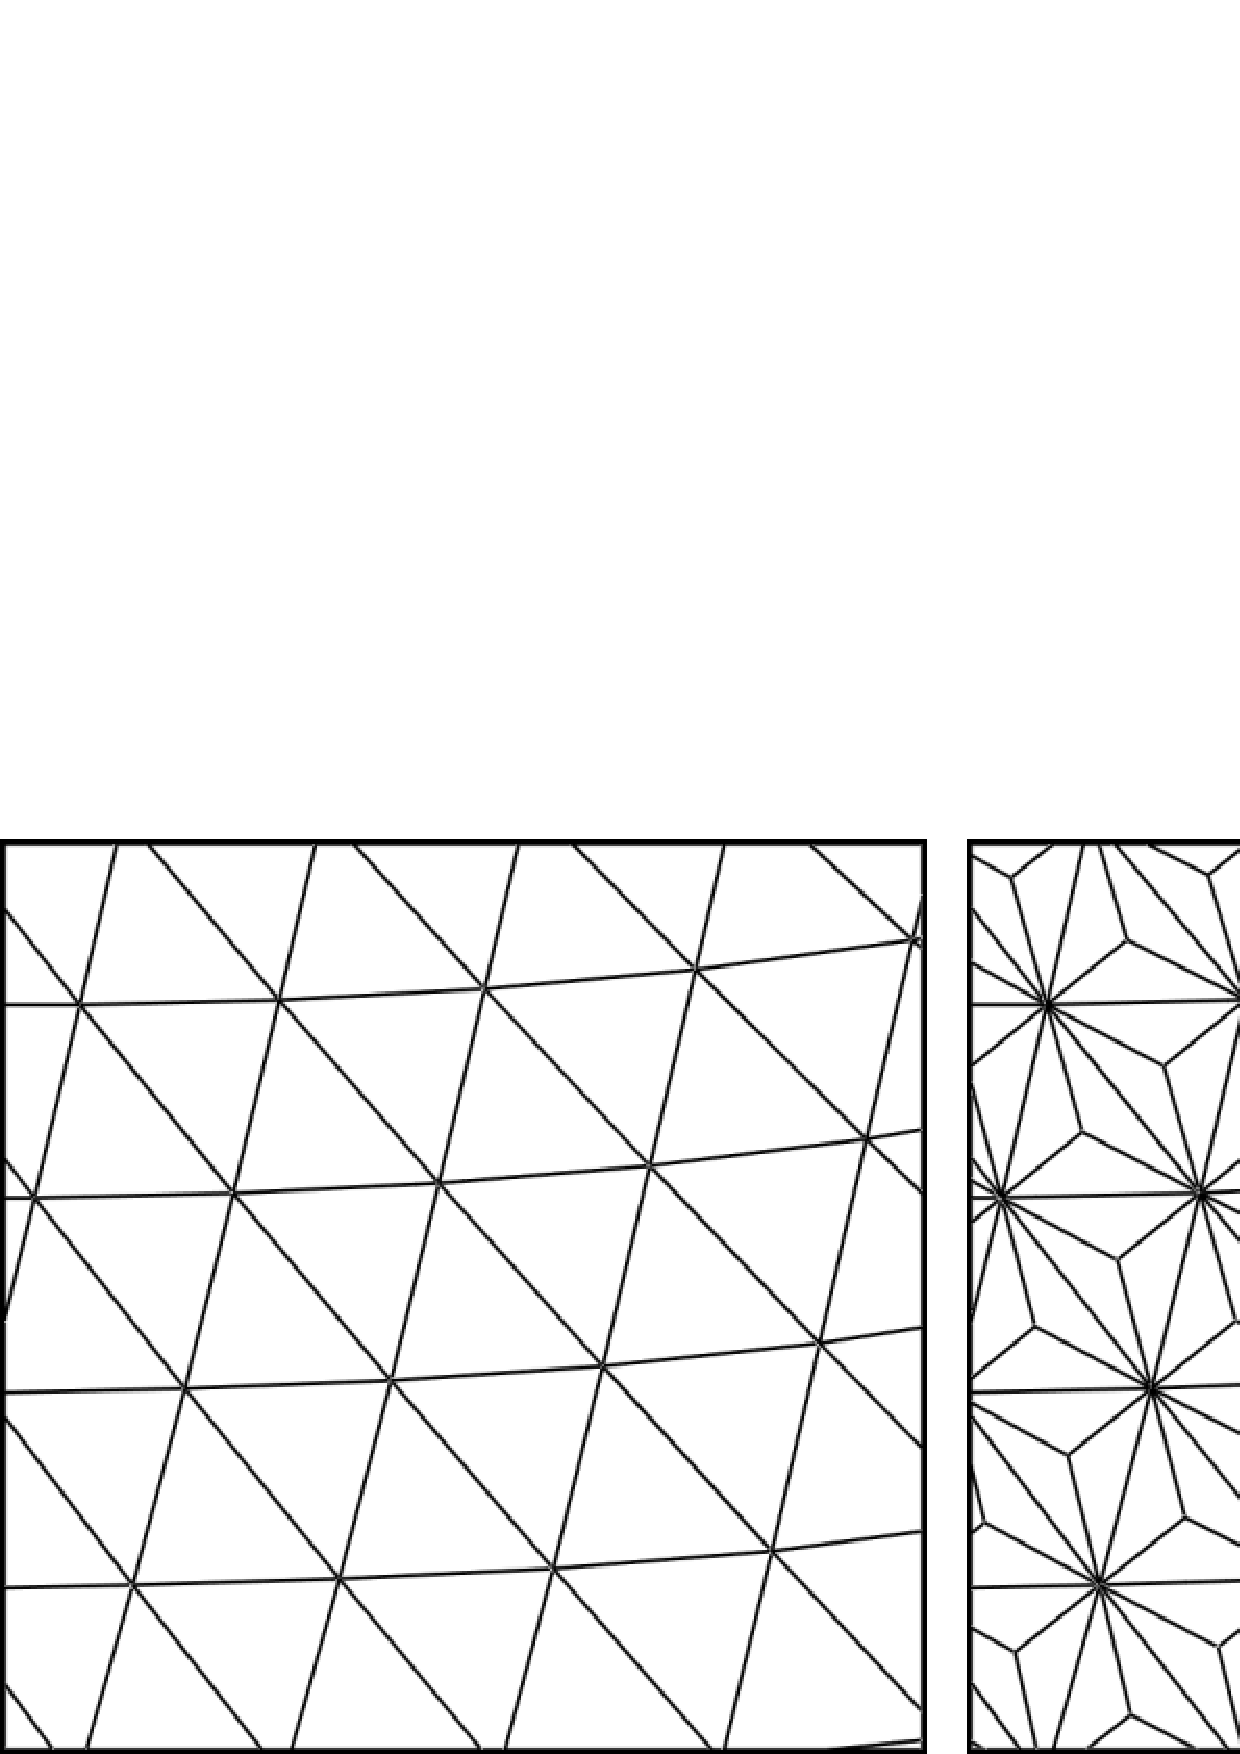
\includegraphics[width=\linewidth]{figs/sqrt3_basic}}
    \caption{The $\sqrt{3}$-Subdivision scheme is decomposed as
             a set of Euler operators: face splits and edge flips.}
    \label{fig:sqrt3_basic}
\end{figure}

{ \scriptsize
\begin{verbatim}

template <class Polyhedron,class kernel>
class CSubdivider_sqrt3
{
	typedef typename kernel::Point_3 Point;
  typedef typename kernel::Vector_3 Vector;
  typedef typename Polyhedron::Vertex                                   Vertex;
  typedef typename Polyhedron::Vertex_iterator                          Vertex_iterator;
  typedef typename Polyhedron::Halfedge_handle                          Halfedge_handle;
  typedef typename Polyhedron::Edge_iterator                            Edge_iterator;
  typedef typename Polyhedron::Facet_iterator                           Facet_iterator;
  typedef typename Polyhedron::Halfedge_around_vertex_const_circulator  HV_circulator;
  typedef typename Polyhedron::Halfedge_around_facet_circulator         HF_circulator;
  typedef typename kernel::FT                                           FT;
  #define PI 3.1415926535897932

public:
  CSubdivider_sqrt3() {}
  ~CSubdivider_sqrt3() {}

  //*********************************************
  // Subdivision
  //*********************************************
  int subdivide(Polyhedron &P,
                int iter)
  {
    // check for valid polygon mesh
    if(P.size_of_facets() == 0)
      return false;

    // normalize border
    P.normalize_border();

    for(int i=0;i<iter;i++)
    {
      // subdivision
      subdivide(P);

       // boundary subdivision
      if(i & 1)
        subdivide_border(P);
    }
    return true;
  }

  ///////////////////////////////////////////////
  // PRIVATE
  ///////////////////////////////////////////////


  //*********************************************
  // Flip edge
  //*********************************************
  void flip_edge(Polyhedron& P,
                 Halfedge_handle e)
  {
    if(e->is_border_edge())
      return;
    Halfedge_handle h = e->next();
    P.join_facet( e);
    P.split_facet( h, h->next()->next());
  }

  //*********************************************
  // Subdivide
  //*********************************************
  void subdivide(Polyhedron& P)
  {
    // We use that new vertices/halfedges/facets are appended at the end.
    std::size_t nv = P.size_of_vertices();
    Vertex_iterator last_v = P.vertices_end();
    -- last_v;  // the last of the old vertices
    Edge_iterator last_e = P.edges_end();
    -- last_e;  // the last of the old edges
    Facet_iterator last_f = P.facets_end();
    -- last_f;  // the last of the old facets

    // create new center vertices
    Facet_iterator f = P.facets_begin();    
    do {
        create_center_vertex( P, f);
    } while ( f++ != last_f);

    std::vector<Point> pts;
    // smooth the old vertices
    pts.reserve( nv);  // get intermediate space for the new points
    ++ last_v; // make it the past-the-end position again
    std::transform( P.vertices_begin(), last_v, std::back_inserter( pts),
                    Smooth_old_vertex());
    std::copy( pts.begin(), pts.end(), P.points_begin());

    Edge_iterator e = P.edges_begin();
    // flip the old edges
    ++ last_e; // make it the past-the-end position again
    while ( e != last_e) {
        Halfedge_handle h = e;
        ++e; // careful, incr. before flip since
             // flip destroys current edge
        flip_edge( P, h);
    };
    CGAL_postcondition( P.is_valid());
  }

  //*********************************************
  // Trisect border halfedge
  //*********************************************
  void trisect_border_halfedge(Polyhedron& P,
                               Halfedge_handle e)
  {
    CGAL_precondition( e->is_border());
    // Create two new vertices on e.
    e = e->prev();
    P.split_vertex( e, e->next()->opposite());
    P.split_vertex( e, e->next()->opposite());
    e = e->next();
    // We use later for the smoothing step that e->next()->next()
    // is our original halfedge we started with, i.e., its vertex is
    // from the unrefined mesh.  Split the face twice.
    Halfedge_handle h = e->opposite()->next();
    P.split_facet( e->next()->next()->opposite(), h);
    P.split_facet( e->next()->opposite(), h);
  }

  //*********************************************
  // Subdivide border
  //*********************************************
  void subdivide_border(Polyhedron& P)
  {
    if ( P.size_of_facets() == 0)
        return;
    // We use that new halfedges are appended at the end.
    Edge_iterator last_e = P.edges_end();
    -- last_e;  // the last of the old edges
    Edge_iterator e = P.edges_begin(); // create trisected border edges
    do {
        if ( e->opposite()->is_border())
            trisect_border_halfedge( P, e->opposite());
        else if ( e->is_border())
            trisect_border_halfedge( P, e);
    } while ( e++ != last_e);
    e = P.edges_begin();     // smooth points on border edges
    std::vector<Point> pts;  // store new smoothed points temporarily
    do {
        if ( e->opposite()->is_border())
            smooth_border_vertices( e->opposite(), std::back_inserter(pts));
        else if ( e->is_border())
            smooth_border_vertices( e, std::back_inserter(pts));
    } while ( e++ != last_e);
    e = P.edges_begin(); // copy smoothed points back
    std::vector<Point>::iterator i = pts.begin();
    do {
        if ( e->opposite()->is_border()) {
            e->vertex()->point() = *i++;
            e->opposite()->vertex()->point() = *i++;
            e->opposite()->next()->vertex()->point() = *i++;
        } else if ( e->is_border()) {
            e->opposite()->vertex()->point() = *i++;
            e->vertex()->point() = *i++;
            e->next()->vertex()->point() = *i++;
        }
    } while ( e++ != last_e);
    CGAL_assertion( i == pts.end());
    CGAL_postcondition( P.is_valid());
  }

  //*********************************************
  // Create center vertex
  //*********************************************
  void create_center_vertex(Polyhedron& P,
                            Facet_iterator f)
  {
    Vector vec( 0.0, 0.0, 0.0);
    std::size_t order = 0;
    HF_circulator h = f->facet_begin();
    do {
        vec = vec + ( h->vertex()->point() - CGAL::ORIGIN);
        ++ order;
    } while ( ++h != f->facet_begin());
    CGAL_assertion( order >= 3); // guaranteed by definition of Polyhedron
    Point center =  CGAL::ORIGIN + (vec / (FT)order);
    Halfedge_handle new_center = P.create_center_vertex( f->halfedge());
    new_center->vertex()->point() = center;
  }

  struct Smooth_old_vertex
  {
     Point operator()( const Vertex& v) const
     {
       std::size_t degree = CGAL::circulator_size( v.vertex_begin());
       if ( degree & 1) // odd degree only at border vertices
           return v.point();
       degree = degree / 2;
       FT alpha = (4.0f - 2.0f * (FT)cos( 2.0f * PI / (FT)degree)) / 9.0f;
       Vector vec = (v.point() - CGAL::ORIGIN) * ( 1.0f - alpha);
       HV_circulator h = v.vertex_begin();
       do {
         // Even degree and border edges indicated non-manifold
         // vertex with two holes.
         if( h->is_border())
         {
           std::cerr << "Error: non-manifold vertex. Erroneous smoothing."
                     << std::endl;
           return v.point();
         }
         vec = vec + ( h->opposite()->vertex()->point() - CGAL::ORIGIN)
           * alpha / (FT)degree;
         ++ h;
         CGAL_assertion( h != v.vertex_begin()); // even degree guaranteed
         ++ h;
       } while ( h != v.vertex_begin());
       return (CGAL::ORIGIN + vec);
     }
  };

  template <class OutputIterator>
  void smooth_border_vertices(Halfedge_handle e,OutputIterator out)
  {
    CGAL_precondition( e->is_border());
    // We know that the vertex at this edge is from the unrefined mesh.
    // Get the locus vectors of the unrefined vertices in the neighborhood.
    Vector v0 = e->prev()->prev()->opposite()->vertex()->point() -CGAL::ORIGIN;
    Vector v1 = e->vertex()->point() - CGAL::ORIGIN;
    Vector v2 = e->next()->next()->next()->vertex()->point() - CGAL::ORIGIN;
    *out++ = CGAL::ORIGIN + (10.0 * v0 + 16.0 * v1 +        v2) / 27.0;
    *out++ = CGAL::ORIGIN + ( 4.0 * v0 + 19.0 * v1 +  4.0 * v2) / 27.0;
    *out++ = CGAL::ORIGIN + (       v0 + 16.0 * v1 + 10.0 * v2) / 27.0;
  }
};
\end{verbatim}}

% sqrt3 subdivision 

\begin{figure}[htb]
    \centering{\includegraphics[width=\linewidth]{figs/sqrt3}}
    \caption{$\sqrt{3}$-Subdivision of the mannequin mesh.}
    \label{fig:sqrt3}
\end{figure}


\subsection{Quad-triangle Subdivision using Incremental Builder}

\label{sec:subdivision_builder}

The quad-triangle subdivision scheme was introduced by
Levin~\cite{l-pg-03}, then Stam and Loop~\cite{sl-qts-02}. It applies
to polygon meshes and basically features Loop subdivision on triangles
and Catmull-Clark subdivision on polygons of the control mesh (see
Fig.\ref{fig:quad-triangle}). After one iteration of subdivision the
subdivided model is only composed of triangles and quads. A simple
solution for implementing such a scheme is to use the
\italic{incremental builder} concept featured by CGAL 
Polyhedron (see Section~\ref{sec:builder}).


% quad-triangle subdivision scheme

\begin{figure}[htb]
    \centering{\includegraphics[width=\linewidth]{figs/quad-triangle}}
    \caption{Quad-triangle subdivision scheme.}
    \label{fig:quad-triangle}
\end{figure}

Subdivision engine

{ \scriptsize
\begin{verbatim}

#include "enriched_polyhedron.h"
#include "builder.h"

template <class HDS,class Polyhedron,class kernel>
class CModifierQuadTriangle : public CGAL::Modifier_base<HDS>
{
private:
  typedef typename kernel::FT           FT;
  typedef typename HDS::Vertex          Vertex;
  typedef typename Vertex::Point        Point;
  typedef typename HDS::Face_handle     Face_handle;
  typedef typename HDS::Halfedge_handle Halfedge_handle;
  typedef typename CGAL::Enriched_polyhedron_incremental_builder_3<HDS> builder;
  typedef typename Polyhedron::Halfedge_around_vertex_circulator Halfedge_around_vertex_circulator;
  typedef typename Polyhedron::Facet_handle Facet_handle;
  typedef typename Polyhedron::Vertex_handle Vertex_handle;

  Polyhedron *m_pMesh;

public:

  // life cycle
  CModifierQuadTriangle(Polyhedron *pMesh)
  {
    CGAL_assertion(pMesh != NULL);
    m_pMesh = pMesh;
  }
  ~CModifierQuadTriangle() {}

  // subdivision
  void operator()( HDS& hds)
  {
    builder B(hds,true);
    B.begin_surface(3,1,6);
      add_vertices(B);
      add_facets(B);
    B.end_surface();
  }

private:
  
  //***************************************************
  // add vertices
  //***************************************************
  void add_vertices(builder &B)
  {
    // put original vertices
    int index = 0;
    typename Polyhedron::Vertex_iterator pVertex;
    for(pVertex = m_pMesh->vertices_begin();
        pVertex != m_pMesh->vertices_end();
        pVertex++)
    {
      pVertex->tag(index);
      B.add_vertex(pVertex->point());
      index++;
    }

    // as many as #edges
    m_pMesh->tag_halfedges(-1);
    typename Polyhedron::Halfedge_iterator pHalfedge;
    for(pHalfedge = m_pMesh->halfedges_begin();
        pHalfedge != m_pMesh->halfedges_end();
        pHalfedge++)
    {
      if(pHalfedge->tag() != -1)
        continue;

      // simple edge bissection
      const Point& p1 = pHalfedge->vertex()->point();
      const Point& p2 = pHalfedge->opposite()->vertex()->point();
      Point point = Point(0.5f*(p1.x()+p2.x()),
                          0.5f*(p1.y()+p2.y()),
                          0.5f*(p1.z()+p2.z()));
      B.add_vertex(point);

      // put vertex indices on both halfedges
      pHalfedge->tag(index);
      pHalfedge->opposite()->tag(index);
      index++;
    }

    // and as many as #facets with degree > 3
    m_pMesh->tag_facets(-1);
    typename Polyhedron::Facet_iterator pFacet;
    for(pFacet = m_pMesh->facets_begin();
        pFacet != m_pMesh->facets_end();
        pFacet++)
    {
      unsigned int degree = Polyhedron::degree(pFacet);
      CGAL_assertion(degree >= 3);
      // forget about triangles, they are
      // simply 1-to-4 subdivided by edge bisection
      if(degree == 3)
        continue; 

      // barycentric subdivision
      Point barycenter;
	    m_pMesh->compute_facet_center(pFacet,barycenter);
      B.add_vertex(barycenter);
      pFacet->tag(index);
      index++;
    }
  }

  //***************************************************
  // add facets
  //***************************************************
  void add_facets(builder &B)
  {
    typename Polyhedron::Facet_iterator pFacet;
    for(pFacet = m_pMesh->facets_begin();
        pFacet != m_pMesh->facets_end();
        pFacet++)
    {
      unsigned int degree = Polyhedron::degree(pFacet);
      CGAL_assertion(degree >= 3);

      if(degree == 3)
      {
        typename Polyhedron::Halfedge_handle pHalfedge = pFacet->halfedge();
        int i0 = pHalfedge->tag();
        int i1 = pHalfedge->vertex()->tag();
        int i2 = pHalfedge->next()->tag();
        int i3 = pHalfedge->next()->vertex()->tag();
        int i4 = pHalfedge->next()->next()->tag();
        int i5 = pHalfedge->next()->next()->vertex()->tag();
        CGAL_assertion(i0 >= 0);
        CGAL_assertion(i1 >= 0);
        CGAL_assertion(i2 >= 0);
        CGAL_assertion(i3 >= 0);
        CGAL_assertion(i4 >= 0);
        CGAL_assertion(i5 >= 0);

        // create 4 triangles
        B.begin_facet();
          B.add_vertex_to_facet(i1);
          B.add_vertex_to_facet(i2);
          B.add_vertex_to_facet(i0);
        const Halfedge_handle& h1 = B.end_facet();
        B.begin_facet();
          B.add_vertex_to_facet(i3);
          B.add_vertex_to_facet(i4);
          B.add_vertex_to_facet(i2);
        const Halfedge_handle& h2 = B.end_facet();
        B.begin_facet();
          B.add_vertex_to_facet(i5);
          B.add_vertex_to_facet(i0);
          B.add_vertex_to_facet(i4);
        const Halfedge_handle& h3 = B.end_facet();

        // center face
        B.begin_facet();
          B.add_vertex_to_facet(i0);
          B.add_vertex_to_facet(i2);
          B.add_vertex_to_facet(i4);
        Halfedge_handle h4 = B.end_facet();

        h1->control_edge(false);
        h1->next()->control_edge(false);
        h1->next()->next()->control_edge(false);

        h2->control_edge(false);
        h2->next()->control_edge(false);
        h2->next()->next()->control_edge(false);

        h3->control_edge(false);
        h3->next()->control_edge(false);
        h3->next()->next()->control_edge(false);

        h4->control_edge(false);
        h4->next()->control_edge(false);
        h4->next()->next()->control_edge(false);
        
        if(pHalfedge->control_edge())
        {
          h1->control_edge(true);
          h3->next()->control_edge(true);
        }
        if(pHalfedge->next()->control_edge())
        {
          h1->next()->control_edge(true);
          h2->control_edge(true);
        }
        if(pHalfedge->next()->next()->control_edge())
        {
          h2->next()->control_edge(true);
          h3->control_edge(true);
        }
      }
      else
      {
        // i1: index of barycenter vertex
        int i1 = pFacet->tag();
        CGAL_assertion(i1 >= 0);

        // for each halfedge
        typename Polyhedron::Halfedge_around_facet_circulator h;
        h = pFacet->facet_begin();
        do
        {
          // i2,3,4: indices of three consecutive
          // vertices on halfedges
          int i2 = h->tag();
          int i3 = h->vertex()->tag();
          int i4 = h->next()->tag();
          CGAL_assertion(i2 >= 0);
          CGAL_assertion(i3 >= 0);
          CGAL_assertion(i4 >= 0);

          // create a quad
          B.begin_facet();
            B.add_vertex_to_facet(i3);
            B.add_vertex_to_facet(i4);
            B.add_vertex_to_facet(i1);
            B.add_vertex_to_facet(i2);
          const Halfedge_handle& pNewHalfedge = B.end_facet();

          pNewHalfedge->control_edge(false);
          pNewHalfedge->next()->control_edge(false);
          pNewHalfedge->next()->next()->control_edge(false);
          pNewHalfedge->next()->next()->next()->control_edge(false);

          if(h->control_edge())
            pNewHalfedge->control_edge(true);
          if(h->next()->control_edge())
            pNewHalfedge->next()->control_edge(true);
        }
        while(++h != pFacet->facet_begin());
      }
    }
  }

  //***************************************************
  // correcting factor
  //***************************************************
	static float correcting_factor(unsigned int ne,
		                             unsigned int nq)
  {
    if(ne == 2 && nq == 1)
      return -0.20505f;
    if(ne == 3 && nq == 1)
      return 0.80597f;
    if(ne == 3 && nq == 2)
      return 0.61539f;
    if(ne == 4 && nq == 1)
      return 0.34792f;
    if(ne == 4 && nq == 2)
      return 0.21380f;
    if(ne == 4 && nq == 3)
      return 0.10550f;
    return 0.0f;
  }
public:  
  //***************************************************
  // smooth vertex positions
  //***************************************************
  static void smooth(Polyhedron *pMesh,
                     bool smooth_boundary = true)
  {
    CGAL_assertion(pMesh != NULL);

    // alloc position vectors
    unsigned int nb_vertices = pMesh->size_of_vertices();
    FT *pPos = new FT[3*nb_vertices];
    CGAL_assertion(pPos != NULL);

    // compute new positions
    unsigned int index = 0;
    typename Polyhedron::Vertex_iterator pVertex;
    for(pVertex = pMesh->vertices_begin();
        pVertex != pMesh->vertices_end();
        pVertex++)
    {
      // border vertices will not move
      if(Polyhedron::is_border(pVertex))
      {
        // do not smooth it
        const Point& curr = pVertex->point();
        if(!smooth_boundary)
        {
          pPos[3*index]   = curr.x();
          pPos[3*index+1] = curr.y();
          pPos[3*index+2] = curr.z();
        }
        // smooth using [1/4 1/2 1/4] cubic B-spline averaging mask
        else 
        {
          const typename Polyhedron::Halfedge_handle& pHalfedge =
            pMesh->get_border_halfedge(pVertex);
          CGAL_assertion(pHalfedge != NULL);
          const Point& next = pHalfedge->vertex()->point();
          const Point& prev = pHalfedge->prev()->prev()->vertex()->point();
          pPos[3*index]   = 0.25f*prev.x() + 0.5f*curr.x() + 0.25f*next.x();
          pPos[3*index+1] = 0.25f*prev.y() + 0.5f*curr.y() + 0.25f*next.y();
          pPos[3*index+2] = 0.25f*prev.z() + 0.5f*curr.z() + 0.25f*next.z();
        }
      } // end is border
      else
      {

        unsigned int nb_quads = 0;
        unsigned int nb_edges = 0;

        // rotate around vertex to count #edges and #quads
        Halfedge_around_vertex_circulator
          pHalfEdge = pVertex->vertex_begin();
        Halfedge_around_vertex_circulator end = pHalfEdge;
        CGAL_For_all(pHalfEdge,end)
        {
          const Facet_handle& pFacet = pHalfEdge->facet();
          CGAL_assertion(pFacet != NULL);
          unsigned int degree = Polyhedron::degree(pFacet);
          CGAL_assertion(degree == 4 || degree == 3);
          if(degree == 4)
            nb_quads++;
          nb_edges++;
        }

        // compute coefficients
        FT ne = (FT)nb_edges;
        FT nq = (FT)nb_quads;
        FT alpha = 1.0f / (1.0f + ne/2.0f + nq/4.0f);
        FT beta = alpha / 2.0f;  // edges
        FT gamma = alpha / 4.0f; // corners of incident quads
        FT eta = correcting_factor(nb_edges,nb_quads);

        // new position
        pPos[3*index]   = alpha * pVertex->point().x();
        pPos[3*index+1] = alpha * pVertex->point().y();
        pPos[3*index+2] = alpha * pVertex->point().z();

        // rotate around vertex to compute new position
        pHalfEdge = pVertex->vertex_begin();
        end = pHalfEdge;
        CGAL_For_all(pHalfEdge,end)
        {
          const Facet_handle& pFacet = pHalfEdge->facet();
          CGAL_assertion(pFacet != NULL);
          unsigned int degree = Polyhedron::degree(pFacet);
          CGAL_assertion(degree == 4 || degree == 3);

          // add edge-vertex contribution
          const Point& point = pHalfEdge->prev()->vertex()->point();
          pPos[3*index]   += beta * point.x();
          pPos[3*index+1] += beta * point.y();
          pPos[3*index+2] += beta * point.z();

          // add corner vertex contribution
          if(degree == 4)
          {
            const Point& corner = pHalfEdge->next()->next()->vertex()->point();
            pPos[3*index]   += gamma * corner.x();
            pPos[3*index+1] += gamma * corner.y();
            pPos[3*index+2] += gamma * corner.z();
          }
        }

        // apply correction
        pPos[3*index] = pPos[3*index] +
          eta*(pPos[3*index]-pVertex->point().x());
        pPos[3*index+1] = pPos[3*index+1] +
          eta*(pPos[3*index+1]-pVertex->point().y());
        pPos[3*index+2] = pPos[3*index+2] +
          eta*(pPos[3*index+2]-pVertex->point().z());

      } // end !is border
      index++;
    }

    // set new positions
    index = 0;
    for(pVertex = pMesh->vertices_begin();
        pVertex != pMesh->vertices_end();
        pVertex++)
    {
      Point& point = pVertex->point();
      point = Point(pPos[3*index],
                    pPos[3*index+1],
                    pPos[3*index+2]);
      index++;
    }

    // cleanup
    delete [] pPos;
  }
};
\end{verbatim}}

{ \scriptsize
\begin{verbatim}
template <class Polyhedron,class kernel>
class CSubdivider_quad_triangle
{
public:
    typedef typename Polyhedron::HalfedgeDS HalfedgeDS;

public:
  // life cycle
  CSubdivider_quad_triangle() {}
  ~CSubdivider_quad_triangle() {}

public:
  void subdivide(Polyhedron &OriginalMesh,
                 Polyhedron &NewMesh,
                 bool smooth_boundary = true)
  {
    CModifierQuadTriangle<HalfedgeDS,Polyhedron,kernel> 
      builder(&OriginalMesh);

    // delegate construction 
    NewMesh.delegate(builder);

    // smooth
    builder.smooth(&NewMesh,smooth_boundary);
  }
};
\end{verbatim}}

% SurfLab

\subsection{Subdivision using a rule template}

\label{sec:subdivision_rule}

Doo-Sabin, Catmull-Clark, Loop.

% APPLICATION DEMO
\section{Application demo}

List of features, snapshots.

\subsection{Compiling on Windows}

\subsection{Compiling on Linux}

% CONCLUSION
\section{Conclusion}

% REFERENCES
\bibliographystyle{alpha}
\bibliography{tutorial}


\end{document}
